\section{Discussion}
\label{Discussion}
\textbf{FIXME: La conclusione la incorporo come subsection della discussion o la tengo separata? }\\
In this section we discuss the issues, the results and the possible future development of our generator. We also present a use case to show how the generator works on a simple transformation.



\subsection{Use Case}
\label{sec:UseCase}
FIXME, to complete with some pictures. \ref{fig:GeneratorUseCase}
\begin{itemize}
 \item The input model complying with our workflow pattern
 \item Run the Acceleo generation
 \item Create an instance of the Java application process' class and run the runWorkflow() method.
 \item The behaviour is the same as when we run an instance of the BPEL's process 
\end{itemize}

\begin{figure}
  \begin{center}
    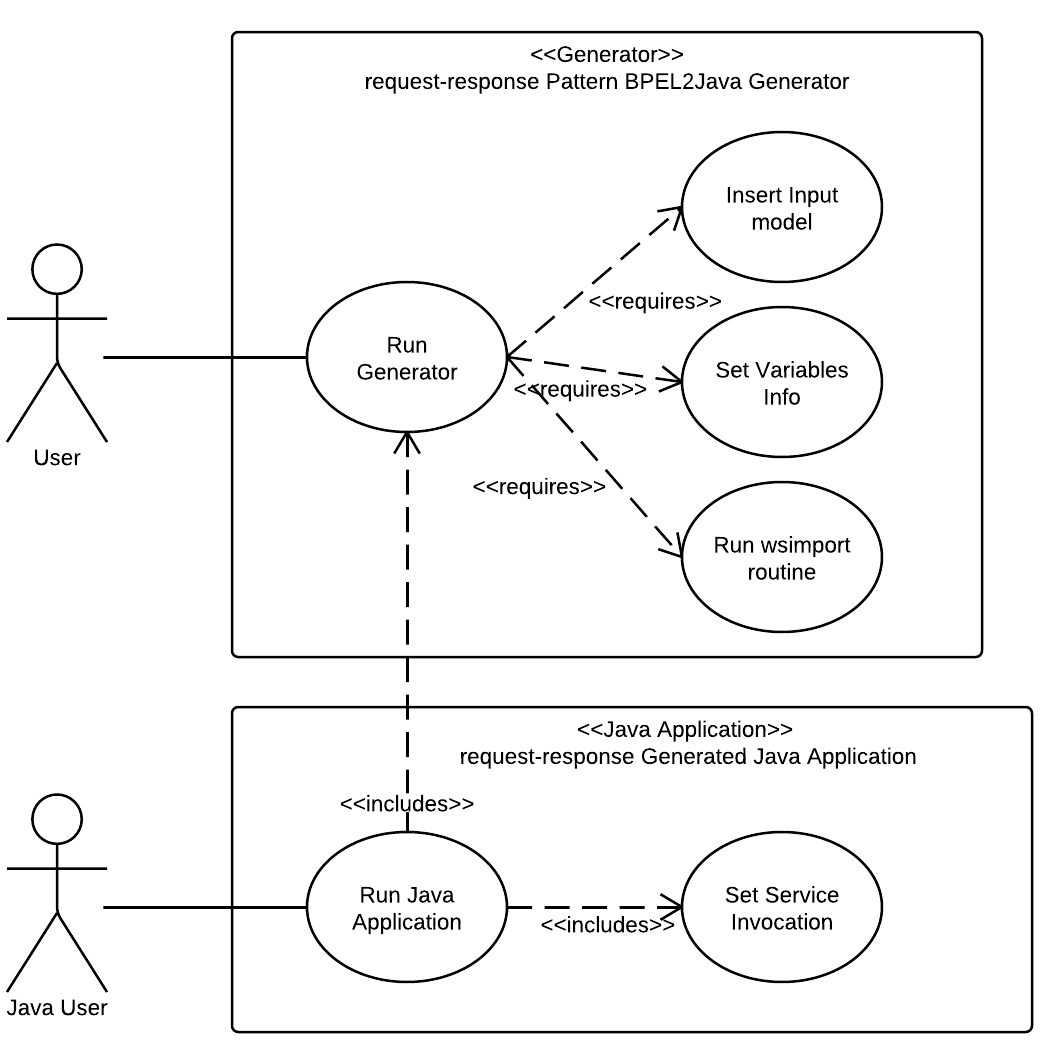
\includegraphics[scale=1.5]{pictures/GeneratorUseCase.png}
    \caption{Use Case}
    \label{fig:GeneratorUseCase}
  \end{center}
\end{figure}



\subsection{Future Development}
\label{sec:FutureDevelopment}
This Section briefly shows the possible improvements and future development that might be carried out on the BPEL to Java transformation.

As previously described in Section \ref{sec:issues}, some technical issues mainly due to the impossibility of providing more than one input models to the Acceleo generator, made us redefine the design and contemplate a developer's intervention 
for anything that concern the WSDL files.
We think that if the information from the WSDL file would be available, the developer's intervention would be much less needed, and error-prone manual operations (like rewriting or copy-pasting the, often long, WSDL elements fields) would be avoided. 
We forecast a possible future development undertaking two ways:
\begin{enumerate}
 \item \label{itm:num1}modify the Acceleo API and implementation
 \item \label{itm:num2}recur to Java properties file 
\end{enumerate}

\paragraph{Modify the Acceleo tool}
Concerning the point number \ref{itm:num1}, modifications to the Acceleo API and its implementation could be made, though at a high cost in terms of time and knowledge to acquire concerning the Acceleo's internal mechanisms. As the Acceleo developers responded us on the official forum, the task would not be a trivial thing.
Moreover, we don't know if the developers would take into considerations the option of rising the number of possible input files. This because the majority of users tend to run the same transformation over several input models of the same kind (e.g. UML diagrams) and a case where coordination is required (BPEL and WSDL files) is not the most common  

For this purpose we contacted the Acceleo developers on the official forum \cite{acceleoForum} to know how to add this possibility. The answer has been that, although possible, it would concern modifying most of the Acceleo API and rewrite the implementation of many methods. So, it would have been not a trivial task.


% FIXME: Modify the list of topics here:
% \begin{itemize}
%  \item Acceleo cannot get more than one input file, that means we cannot read the information from the WSDL file(s).
%   \subitem The variables types have to be input manually
%   \subitem The "assign" activities cannot be translated automatically
%   \subitem The infos to invoke a real web service are inside the WSDL file
%  \item solutions:
%   \subitem Modify Acceleo API, or wait for Acceleo to support this thing.
%   \subsubitem We tried to talk with the Acceleo developers but it was not time wise feasible task
%   \subitem Un'idea per sormontarli sarebbe di andare a creare un'altra trasformazione Acceleo, che dato in input un file WSDL, scrive le informazioni necessarie in un file Java-properties che verrà poi usato dall'applicazione Java. Se i file WSDL sono più di uno, la trasformazione viene eseguita più volte (a seconda del numero dei file WSDL) andando ad aggiungere altre linee nel file Java-properties
% \end{itemize}
